%%%%%%%%%%%%%%%%%%%%%%%%%%%%%%%%%%%%%%%%%%%%%%%%
%%%%%%%%%%%%%%%%%%%%%%%%%%%%%%%%%%%%%%%%%%%%%%%%
%
%		Kommentar
%		Ein nettes old school template.......
%		last modified: 27/03/07
%
%%%%%%%%%%%%%%%%%%%%%%%%%%%%%%%%%%%%%%%%%%%%%%%%
%%%%%%%%%%%%%%%%%%%%%%%%%%%%%%%%%%%%%%%%%%%%%%%%
\documentclass[a4paper,11pt,oneside]{scrartcl}
\usepackage{eurosym}
\usepackage[german]{babel}
\usepackage{amsmath}
\usepackage{amssymb}
\usepackage[automark]{scrpage2}	%Kopfzeile Autoinhalt (Kapitel)
\usepackage{graphics}
\usepackage{color}
\usepackage{graphicx}
\usepackage{longtable}
\usepackage{lscape}
\usepackage{hhline}
\usepackage{booktabs}
\usepackage{IFSlogo}
\usepackage{multirow}
% \usepackage[T1]{fontenc}
% \usepackage[pdftex]{hyperref}
\usepackage{makeidx}
% \selectlanguage{english}
\setlength{\parindent}{0pt}  % setzt sie Einrückung nach einem Umbruch zurück

%%%%%%%%%%%%%%%%%%%%%%%%%%%%%%%%%%%%%%%%%%%%%%%%
%		Sachregister-Erstellung
%		Begriffe werden mit Befehl \index{} aufgenommen
% 		Index erstellen in Konsole makeindex -g -s style.ist Vorlage.idx 
%%%%%%%%%%%%%%%%%%%%%%%%%%%%%%%%%%%%%%%%%%%%%%%% 
\makeindex


%%%%%%%%%%%%%%%%%%%%%%%%%%%%%%%%%%%%%%%%%%%%%%%%
%		ETH-Schrift einführen
%%%%%%%%%%%%%%%%%%%%%%%%%%%%%%%%%%%%%%%%%%%%%%%% 

% \usepackage[standard-baselineskips]{cmbright} % Mathematikschrift die in etwa ETH-Light entspr.
\renewcommand{\sectfont}{\bfseries}

%\renewcommand{\familydefault}{let} 
%\renewcommand{\seriesdefault}{let}
%\renewcommand{\shapedefault}{let}
%\renewcommand{\sfdefault}{let}
\renewcommand{\rmdefault}{let}


% \DeclareFixedFont{\x}{T1}{let}{m}{n}{10}
% \DeclareFixedFont{\xb}{T1}{let}{m}{n}{10}
% \newfont{\xiiiv}{letr8t at 8.0pt}
% \newfont{\xiiivb}{letb8t at 8.0pt}


%%%%%%%%%%%%%%%%%%%%%%%%
% Schriftengefrickel
%%%%%%%%%%%%%%%%%%%%%%%%%
\usepackage{fontspec}
\usepackage{sectsty}

\partfont{\font \x="DINNeuzeitGroteskStd-Light" at 40pt\x}
\chapterfont{\font \x="DINNeuzeitGroteskStd-Light" at 32pt\x}
\sectionfont{\font \x="DINNeuzeitGroteskStd-Light" at 16pt\x}
\subsectionfont{\font \x="DINNeuzeitGroteskStd-Light" at 14pt\x}
\subsubsectionfont{\font \x="DINNeuzeitGroteskStd-Light" at 14pt\x}
\paragraphfont{\font \x="DINNeuzeitGroteskStd-Light" at 14pt\x}
\newfontface\swashed[Contextuals=Swash, Ligatures=Common]{Adobe Garamond Pro Italic}
\newfontface\foo[Numbers={OldStyle},Contextuals=Swash, Ligatures=Common]{Adobe Garamond Pro}
\newfontface\foofat[Numbers={OldStyle},Contextuals=Swash, Ligatures=Common]{Adobe Garamond Pro Bold}


\usepackage[a4paper,left=4.0cm, right=4.0cm,top=3.0cm, bottom=3.0cm]{geometry}
	
%%%%%%%%%%%%%%%%%%%%%%%%%%%%%%%%%%%%%%%%%%%%%%%%
%		eigenen Stil definieren
%%%%%%%%%%%%%%%%%%%%%%%%%%%%%%%%%%%%%%%%%%%%%%%% 
\pagestyle{scrheadings}
% \renewcommand*{\chapterpagestyle}{scrheadings} 
\clearscrheadfoot 
\ihead{\textsf{\headmark}} 
\ohead{\pagemark}
\setheadsepline{.4pt}
\setfootsepline{.4pt}
\ifoot{}
\ofoot{\footnotesize{\textsc{Hsr, Silvio Heuberger}}}


% frickelabst�nde

% abst�nde und sooooo
\setlength{\columnsep}{10mm}
\setlength{\parskip}{2.5mm}

%two column float page must be 90% full
\renewcommand\dblfloatpagefraction{.90}
%two column top float can cover up to 80% of page
\renewcommand\dbltopfraction{.80}
%float page must be 90% full
\renewcommand\floatpagefraction{.90}
%top float can cover up to 80% of page
\renewcommand\topfraction{.80}
%bottom float can cover up to 80% of page
\renewcommand\bottomfraction{.80}
%at least 10% of a normal page must contain text
\renewcommand\textfraction{.1}


%%%%%%%%%%%%%%%%%%%%%%%%%%
% listings for everyone

\definecolor{defgray}{cmyk}{0.3,0.05,0,0.43}
\usepackage[plainpages={false}, bookmarks, pdfstartview={FitV}, colorlinks, linkcolor=defgray]{hyperref}


\usepackage{listings}
\lstset{% general command to set parameter(s)
basicstyle=\ttfamily\small, % print whole listing small
%basicstyle=\small,
commentstyle=\color{defgray}, % comments
stringstyle=\ttfamily, % typewriter type for strings
showstringspaces=false,
keywordstyle=\bfseries\color{blue},
numbers=left,
numberstyle=\color{defgray}\tiny,
frame=single,
%frame=shadowbox,
%frameround=tttt,
rulesepcolor=\color{defgray},
language={ruby}
} % no special string spaces


% make monospace font the same size (optocally) as Arno Pro
\setmonofont[Scale=0.9]{ITC American Typewriter Std Condensed}
\defaultfontfeatures{Scale=MatchLowercase,Mapping=tex-text}

\begin{document}
\renewcommand{\theequation}{\thesection.\arabic}
\addtokomafont{caption}{\small}
\setkomafont{captionlabel}{\sffamily\bfseries}
\numberwithin{equation}{section}
\pagenumbering{Roman}
\setcapindent*{1em}

%%%%%%%%%%%%%%%%%%%%%%%%%%%%%%%%%%%%%%%%%%%%%%%%
%		Titelseite
%%%%%%%%%%%%%%%%%%%%%%%%%%%%%%%%%%%%%%%%%%%%%%%%
\titlehead{
	\begin{minipage}{0.6\textwidth}{\IFSlogo[50mm]}
 	\end{minipage}
	\begin{minipage}{0.4\textwidth}
		\footnotesize \rightline{HSR Rapperswil} \rightline{Institut für Software}
	\end{minipage}
 } 

\author{Silvio Heuberger and Stefan Keller\\ Institut für Software}
\subject{Extended Abstract}
\title{Extending a grid based geocoding system with geospatial functions}
\date{April 2010}
\publishers{}
\dedication{} 
\maketitle


\fontspec[Numbers={OldStyle}, Ligatures={Common}]{Adobe Garamond Pro}
\pagenumbering{arabic}

%%%%%%%%%%%%%%%%%%%%%%%%%%%%%%%%%%%%%%%%%%%%%%%%
%		Ab hier gehts los mit dem Dokument
%%%%%%%%%%%%%%%%%%%%%%%%%%%%%%%%%%%%%%%%%%%%%%%%

\section{Geohash.org} % (fold)
When writing the site \url{geohash.org} in 2008 Gustavo Niemeyer invented the so-called geohash. Initially a geohash was to be used to shorten and simplify the handling of geographic coordinates so they can be used more efficiently in URLs and e-mail. For instance, the point $(47.864500, 8.842342)$ can be represented by the geohash \texttt{u0w231qyct80}.

Because this geohash is acquired by gradually subdividing the latitude and longitude range into smaller boxes, this hash does not actually represent a point, but an arbitrarily small bounding box. One can remove accuracy (i.e. make the bounding box bigger) by removing bits (characters) from the hash. Removing characters from the end of the geohash, yields \texttt{u0w23} which is the bounding box
\[
(47.8564453125,8.8330078125) \rightarrow (47.900390625,8.876953125)
\]
centered around the point $(47.9, 8.9)$.

Since the hash is base32-encoded removing characters will remove multiples of 5 bits.

However when representing the hash as interleaved bits of a long, one can also remove a single bit, i.e. a single subdivision of either the latitude or longitude range.

\section{Encoding a geohash as a \texttt{long}} % (fold)
\label{sec:encoding_a_geohash_as_a_}
The algorithm to encode a coordinate pair $p = (lat,lon)$ into a geohash bounding box works as follows:

\begin{enumerate}
	\item Start with the latitude and longitude ranges $r_{lat} = (-90,90)$ and $r_{lon} = (-180,180)$ and an empty hash with no bits set.
	\item \begin{enumerate}
		\item For even bits, find the arithmetic mean $\hat{lon}$ of $r_{lon}$ and flip the last bit on, if $lon \geq \hat{lon}$. Make the arithmetic mean the new start or end of $r_{lon}$ respectively for the next step.
		\item For odd bits, do the same thing as in (a) but use the range $r_{lat}$ and $lat$.
	\end{enumerate}
	\item Continue at (2) until the desired precision is acquired.
	\item Use a left shift, to align the determined bits at the “front” of the \texttt{long}.
\end{enumerate}

The last step is necessary, in order for the bits to be at the start of the hash, thus enabling a simple mask to be used to extract any prefix of a hash and use it to check wether other hashes lie \emph{within} it.
% section encoding_a_geohash_as_a_ (end)


\section{Maximal bounding box size with 64 bits} % (fold)
\label{sec:maximal_precision_with_64_bits}
We quickly want to establish an approximation of the accuracy such a hash achieves, when representing point data.

If we encode a coordinate pair $p = (9.004046, -79.523453, 64)$ down to the maximal precision that can be obtained by using a \texttt{long} as storage, we end up with the following hash (alas, it cannot be meaningfully represented in base32):

\[
h_p = 110000001111010011110100101111000011010000110010111111011001100
\]

which represents the following bounding box:

\[
(9.004045994952321,-79.52345302328467)
\]
\[
(9.004046036861837,-79.52345293946564)
\]

This hash's bounding box (in Panamà) has a diagonale of about $\approx 0.8084 cm$. Since this is near the equator, bounding boxes that are closer to the poles will only get smaller, for example a 64-bit bounding box in Ystad will yield a diagonale of $\approx 0.70667 cm$.

Having established that a 64-bit \texttt{long} is actually a good approximation as a pretty small bounding box around a coordinate point, we can move on to more interesting facts, for instance proximity of hashes.


\section{Same prefix for larger bounding boxes} % (fold)
\label{sec:same_prefix_for_larger_bounding_boxes}
It can be seen that removing precision from a hash will yield a less precise hash, that includes all the hashes that share the shorter hash as a prefix.
The hash \texttt{u0w231qyct80} is completely \emph{within} all of the following hashes: \texttt{u0w2, u0w231, u0w231qyc}

Subsequently, the hash \texttt{u0w2} \emph{contains} a theoretically infinitely large set of hashes (of course the set of 64-bit hashes is limited, but we don't need to stop there), all sharing the common prefix \texttt{u0w2}.

It can easily be seen that the hash \texttt{bcde} is clearly \emph{not within} \texttt{u0w2}.

Looking at this fact from a “binary perspective”, one can easily see, that the question wether a hash lies within another hash's bounding box simply boils down to a binary operation, based on the prefix of the hash:

TODO: Explain binary operation.

Iff the first bits of the hash are the same as of the bounding box, it is contained within the bounding box.


% section same_prefix_for_larger_bounding_boxes (end)

\section{Similar hashes for nearby points} % (fold)
\label{sec:similar_hashes_for_nearby_pojnts}
Since the geohash is built as an interleaved set of bits for each subsequent latitude or longitude range division, nearby boxes often have similar prefixes. Alas, this is not always the case, because there's also corner cases that cross boundaries that go beyond the prefix of the hash. If we hit a boundary, the hashes might suddenly “flip over” to a rather different prefix. This is especially true around the meridians.

For instance, the point $p = (41.7, 0.08)$ encodes into the following four-character (20-bit) geohash: \texttt{sp2j}.
Out of it's eight neighbouring hashes, only 5 have a similar prefix as can be seen in figure~\ref{fig:4-grid}

\begin{figure}[t]
	\centering
	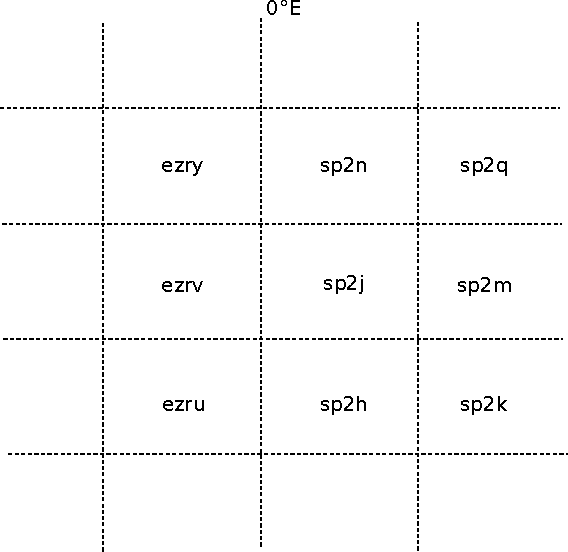
\includegraphics[width=7cm]{graphics/grid_meridian.pdf}
	\caption{The 4-character geohash grid around the point $p = (41.7, 0.08)$}
	\label{fig:4-grid}
\end{figure}

This makes using geohashes for proximity searches a little awkward but not impossible. There's a simple algorithm that will wrap around meridians correctly when calculating neighbouring hashes programatically:

\section{Moving around with hashes} % (fold)
\label{sec:Moving around with hashes}

Finding the nearby hashes might seem awkward at first, but there's a pretty simple way to determine the hash that lies in a specific direction, when starting out with a hash.

\begin{enumerate}
  \item Split the interleaved bits into two seperate numbers $bits_{lat}$ and $bits_{lon}$. Make them right-aligned instead of left-aligned by shifting them right the appropriate number of places.
  \item Depending on the direction you want to find the next hash, add or subtract one from the latitude or longitude bits:
  \begin{enumerate}
    \item North: $bits_{lat} \stackrel{+}{=} 1$
    \item South: $bits_{lat} \stackrel{-}{=} 1$
    \item East: $bits_{lon} \stackrel{+}{=} 1$
    \item West: $bits_{lon} \stackrel{-}{=} 1$
  \end{enumerate}
  \item After this step, recombine the bits in an interleaved fashion.
\end{enumerate}


\section{Size of the bounding boxes for $n$ bits} % (fold)
\label{sec:Size of the bounding boxes for $n$ bits}
There is a simple correlation between the number of bits $n$ and the size $\delta$ of a bounding box in degrees.

\begin{displaymath}
  \delta_{lat} = \frac{180}{2^{\lfloor \frac{n}{2} \rfloor}}
\end{displaymath}

\begin{displaymath}
  \delta_{lon} = \frac{360}{2^{\lfloor \frac{n+1}{2} \rfloor}}
\end{displaymath}

% section Size of the bounding boxes for $n$ bits (end)


\end{document}
